\documentclass{beamer}
\usepackage[export]{adjustbox}
\usetheme{CambridgeUS}
\useoutertheme{infolines}
\usepackage{tikz}
\usepackage{wrapfig}
\graphicspath{ {images/} }
\newcommand\RBox[1]{%
 \tikz\node[draw,rounded corners,align=center] {#1};%
}  
\author[Team LondonSW]
{%
   \texorpdfstring{
        \begin{columns}
            \column{.30\linewidth}
            \RBox{ Violetta Avkhukova}
        \end{columns}
        \begin{columns}
            \column{.30\linewidth}
            \RBox{Yakubu Aliyu Doma}
        \end{columns}
        \begin{columns}
            \column{.30\linewidth}
            \RBox{Rawan Mohammed Alrahili}
        \end{columns}
        \begin{columns}
            \column{.30\linewidth}
            \RBox{Felix Santiago Anda Basabe}
        \end{columns}
        \begin{columns}
            \column{.30\linewidth}
            \RBox{Jia Liu}
        \end{columns}
        \vspace{-0.3cm}
        \begin{columns}
          \column{0.3\linewidth}
          \raggedleft
           \includegraphics[width=2.0 cm]{logo_map}
            \vspace{-3 cm}
            \column{0.6\linewidth}
            \raggedright
            \textbf{7CCSMGPR}\\
            \vspace{-4.8cm}
        \end{columns}
   }
   {}
}
\title{Traffic Simulator}
\begin{document}
\begin{frame}
\titlepage
\end{frame}

  
  \begin{frame}
\frametitle{Aims}
   \begin{itemize}
	\item \textbf{Must}
			\begin{itemize}
			\item{Cellular Automaton}
			\item{Vehicle Entry and Exit}
			\item{ Free Movement and Turning of vehicles}
			\item{Default Map}
			\item{Display Simple Animation of Vehicle Movement}	
		\end{itemize}	
	\item \textbf{Should}
			\begin{itemize}
			\item{Create, Save/Load Maps}
			\item{Traffic Policies - lane disabling, light durations}
			\item{Priorities for  Emergency Services}
		\end{itemize}
\item \textbf{Could}
			\begin{itemize}
			\item{Statistics - time spent at traffic e.t.c}
			\item{Curved Roads}
			\item{External Map Sources, e.g OpenStreetMap}
		\end{itemize}	
	\end{itemize}	
  \end{frame}
  
  \begin{frame}
    \frametitle{Design}
       \begin{itemize}
	    \item \textbf{Cellular Automata}
			\begin{itemize}
			\item{Simple and efficient}
			\item{Realistic simulation}
		\end{itemize}
	\end{itemize}
	
	\begin{itemize}
	\item \textbf{MVC}
	\end{itemize}

	\begin{itemize}
	\item \textbf{Design Patterns}
	\end{itemize}

	
  \end{frame}
  
  	\begin{frame}
	  \frametitle{Design cont....}
	    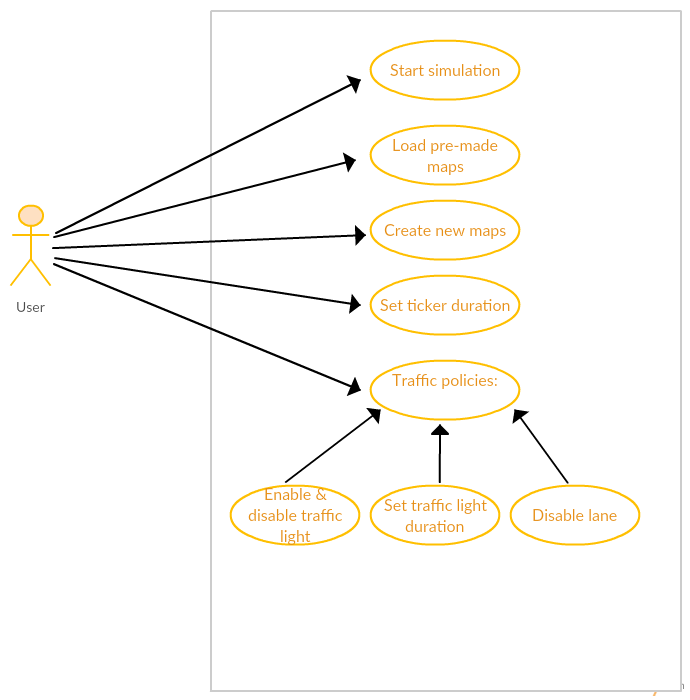
\includegraphics[width=0.50\textwidth, center]{UseCase}
	  
	  \end{frame}

	  \begin{frame}
      	  \frametitle{Iterations}
      	    \frame{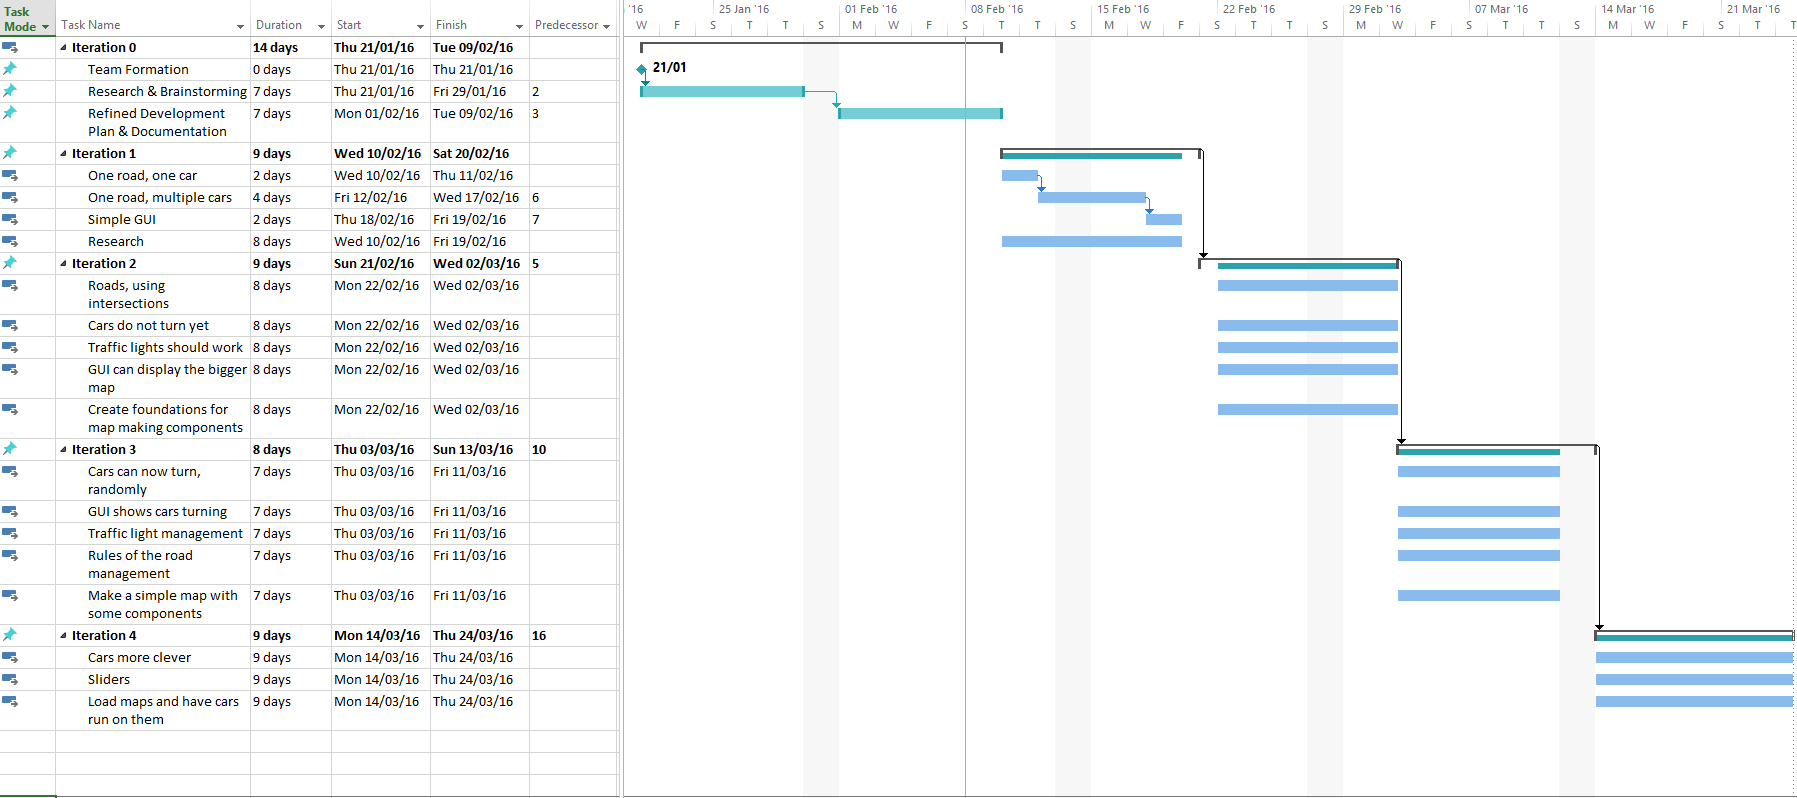
\includegraphics[width=1.0\textwidth, center]{LondonSW_Gantt}}

      	  \end{frame}

       \begin{frame}
      	  \frametitle{Map Structure}
      	     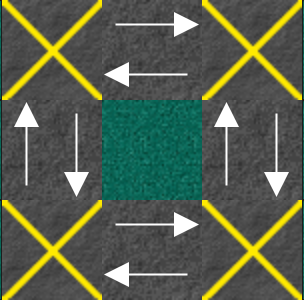
\includegraphics[width=0.5\textwidth, center]{map_structure}
      	  \end{frame}

       \begin{frame}
      	  \frametitle{Testing}
      	    \begin{itemize}
      	    \item Integration Testing
      	    \item JUNIT
      	    \end{itemize}
	 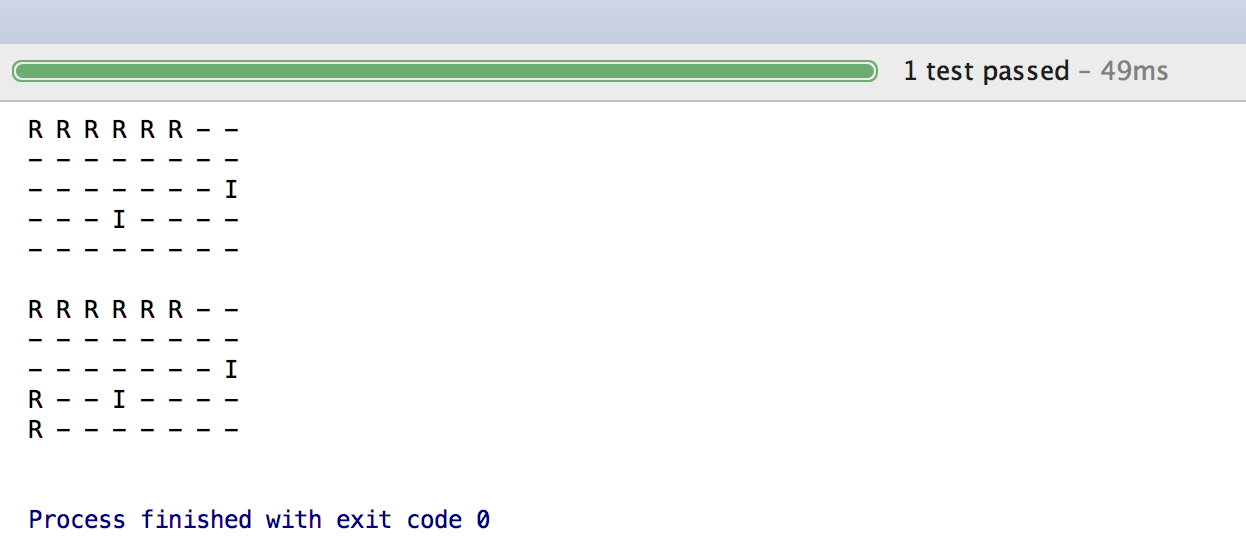
\includegraphics[width=0.5\textwidth, center]{test_mapgrid}
      	  \end{frame}
	  
	  \begin{frame}
      	  \frametitle{Ticker}
      	    \begin{itemize}
      	    \item Keeps track of time in the system
      	    \item Tick Interval
	    \item \textbf{Two implementations:}
	    	\begin{itemize}
	    		\item First implementation:
	    		\begin{itemize}
	    			\item Java Timer
				\item Ran in its own thread
				\item Issues with JavaFX
			\end{itemize}
	    		\item Second implementation:
	    	\begin{itemize}
	    		\item Relies on RxJava, RxJavaFX
	    		\item Ticker = Observable
	    		\item Classes become Subscribers, perform operation onNext(Long l)
	    	\end{itemize}
	    \end{itemize}
      	    \item Tick interval set before simulation start
	    \end{itemize}
      	  \end{frame}

	 \begin{frame}
      	  \frametitle{Traffic Lights}
		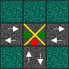
\includegraphics[scale=1, center]{trafficLight}
      	    \begin{itemize}
      	    \item 2 states: red, green
      	    \item Duration
	    \item Subscribe to ticker
	    \item onNext(): change colour when needed
      	    \end{itemize}
      	  \end{frame}

\begin{frame}
\frametitle{Vehicle Class}
\begin{itemize}
\item Vehicle is an abstract class that all vehicles implement.
\item Vehicles have a lot of attributes that are either global or specific.
\item There are two types of vehicles: 
\begin{itemize}
\item Cars.
\item Ambulances.
\end{itemize}

\end{itemize}

\end{frame}
	  
\begin{frame}
\frametitle {Vehicle Movement and Ticker Interaction}
Vehicle movement can be divided into two main categories:
\begin{wrapfigure}{r}{0.35\textwidth}
   \fbox{ 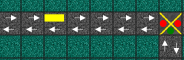
\includegraphics[scale=.5]{lane}}
\end{wrapfigure}
\begin{enumerate}
\item Moving in a lane:
\begin{itemize}
\item Each lane is an array list of vehicles.
\item Vehicles are items in lanes.
\end{itemize}

\item Turning to a new lane
\begin{itemize}
\item Reading traffic light. \texttt {void readTrafficLight()}
\item Choosing lane to move to. \texttt{ Lane chooseLane() }
\item Ability to turn. boolean \texttt{vehicleTurnFirst (ArrayList<Vehicle> vehicles)}
\begin{figure}[h]
\fbox{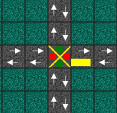
\includegraphics[scale=.5]{intersection}}
\end{figure}
\end{itemize}
\end{enumerate}
Vehicle turns: \texttt{ int vehicleTurn(Lane l) } 

\end{frame}

\begin{frame}
\frametitle{Log}
\begin{itemize}
\item Format Log Year-Month-Day-Hour- Minute-Second
\item Suscribes to ticker
\item Records attributes of each Subscriber
\item Useful for debugging processes, audits, and statistics.
\end{itemize}

\begin{center}
\fbox{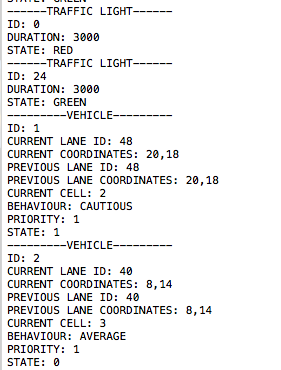
\includegraphics[scale=.4]{logs}}
\end{center}

\end{frame}

\begin{frame}
\frametitle{GUI}
\framesubtitle{Map GUI}

\begin{columns}[T]
 \column{0.99\textwidth}
  \begin{itemize}
   \item Grid of rows and columns
   \item Each cell is a StackPane
   \item Gimp for drawings
   \item Dynamic size: resize factor
  \end{itemize}

 \column{0.01\textwidth}
 \hspace*{-5 cm}
\end{columns}
\begin{center}
 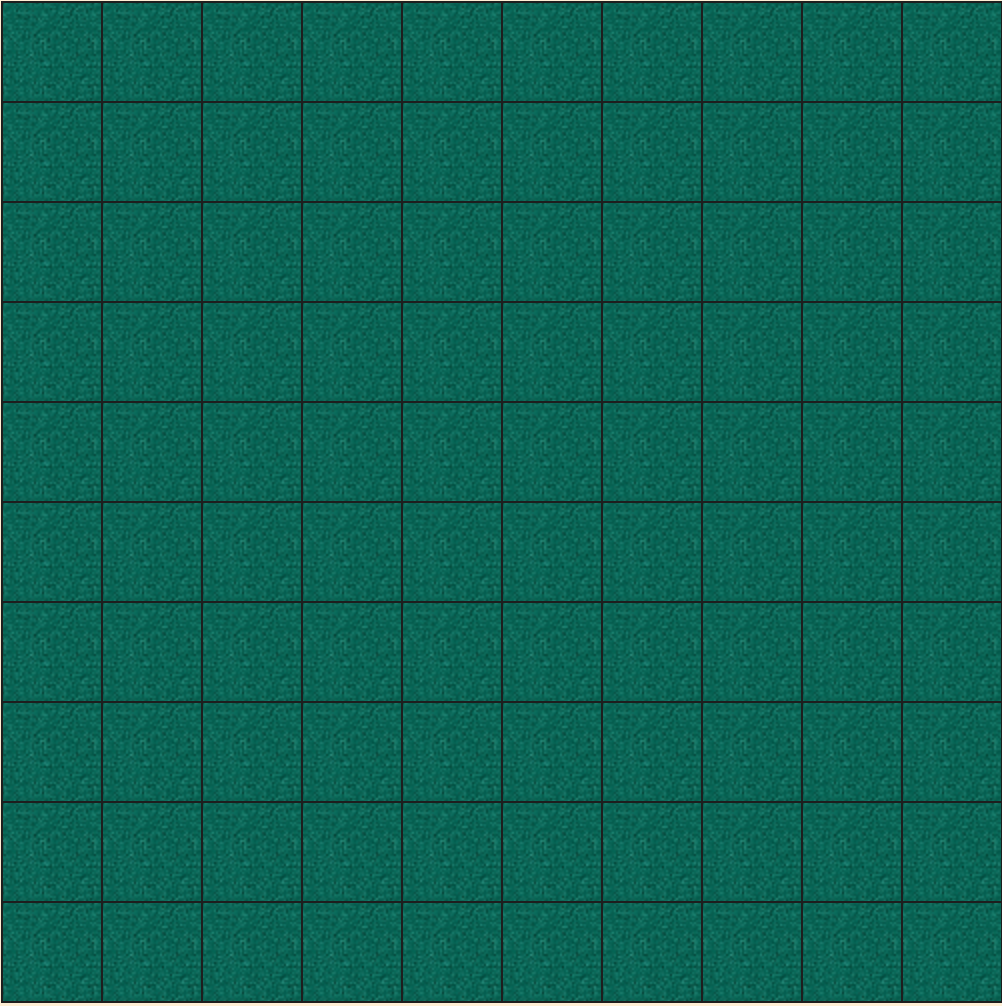
\includegraphics[scale=.2]{gridPane}

\includegraphics[scale=.2]{JavaFX}

\includegraphics[scale=.2]{gimp}
\end{center}

\end{frame}


\begin{frame}
\frametitle{GUI}
\framesubtitle{Decorators}

\begin{itemize}
\item \textbf{MapGridGUIDecorator}
\begin{itemize}
\item Manages the drawing of the entire map
\newline
\end{itemize}
\item \textbf{RoadGUIDecorator}
\begin{itemize}
\item Draws a Road and programatically the lanes
\newline
\end{itemize}
\item \textbf{IntersectionDecorator}
\begin{itemize}
\item Extends the Intersection Functionality 
\newline
\end{itemize}
\item \textbf{TrafficLightDecorator}
\begin{itemize}
\item Circles are drawn programatically
\newline
\end{itemize}
\item \textbf{VehicleGUIDecorator}
\begin{itemize}
\item State [0 to 3]  
\newline
\end{itemize}
\end{itemize}

\end{frame}

\begin{frame}
\frametitle{GUI}
\framesubtitle{Map Simulation}

\begin{center}
\fbox{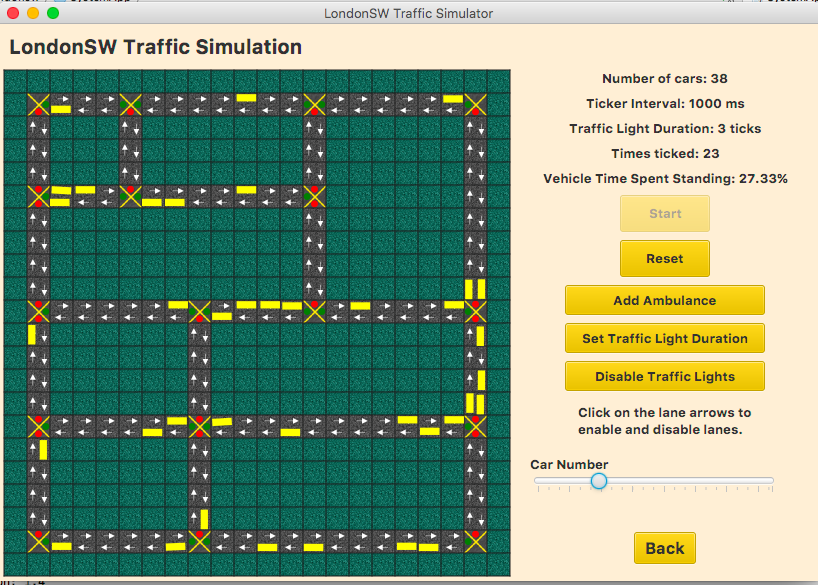
\includegraphics[scale=.3]{map_simulation}}
\end{center}

\end{frame}

\begin{frame}
\frametitle {Map Maker Mode}
Users create their own maps
\begin{wrapfigure}{r}{0.35\textwidth}
   \frame{ 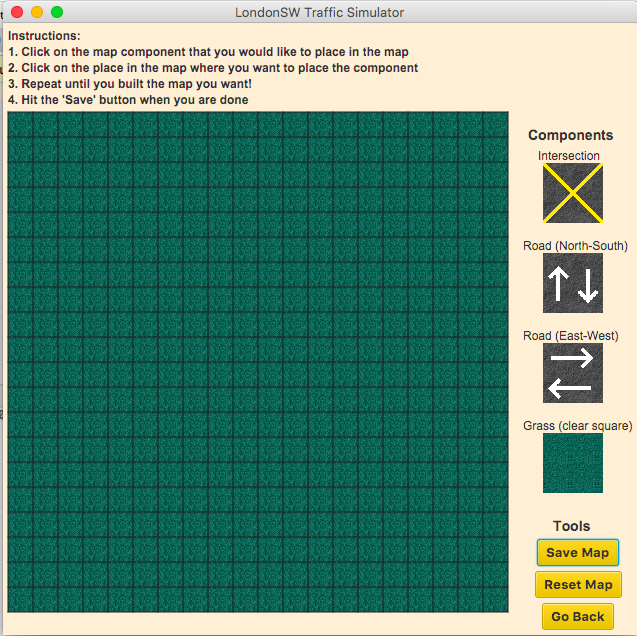
\includegraphics[scale=.15]{mapmaker}}
\end{wrapfigure}
\begin{itemize}
\item Ask for width and height
\item 4 types of map component:
\begin{itemize}
\item intersection
\item road (north-south)
\item road (east-west)
\item grass
\end{itemize}
\item Click on component, click in map any number of times
\item Saving the map
\end{itemize}
\end{frame}

\begin{frame}
\frametitle{Teamwork}
\begin{itemize}
\item Group meeting
\item Agile development with Mingle
\begin{itemize}
\item Mingle's Planner feature
\end{itemize}
\end{itemize}
\begin{figure}[h]
\fbox{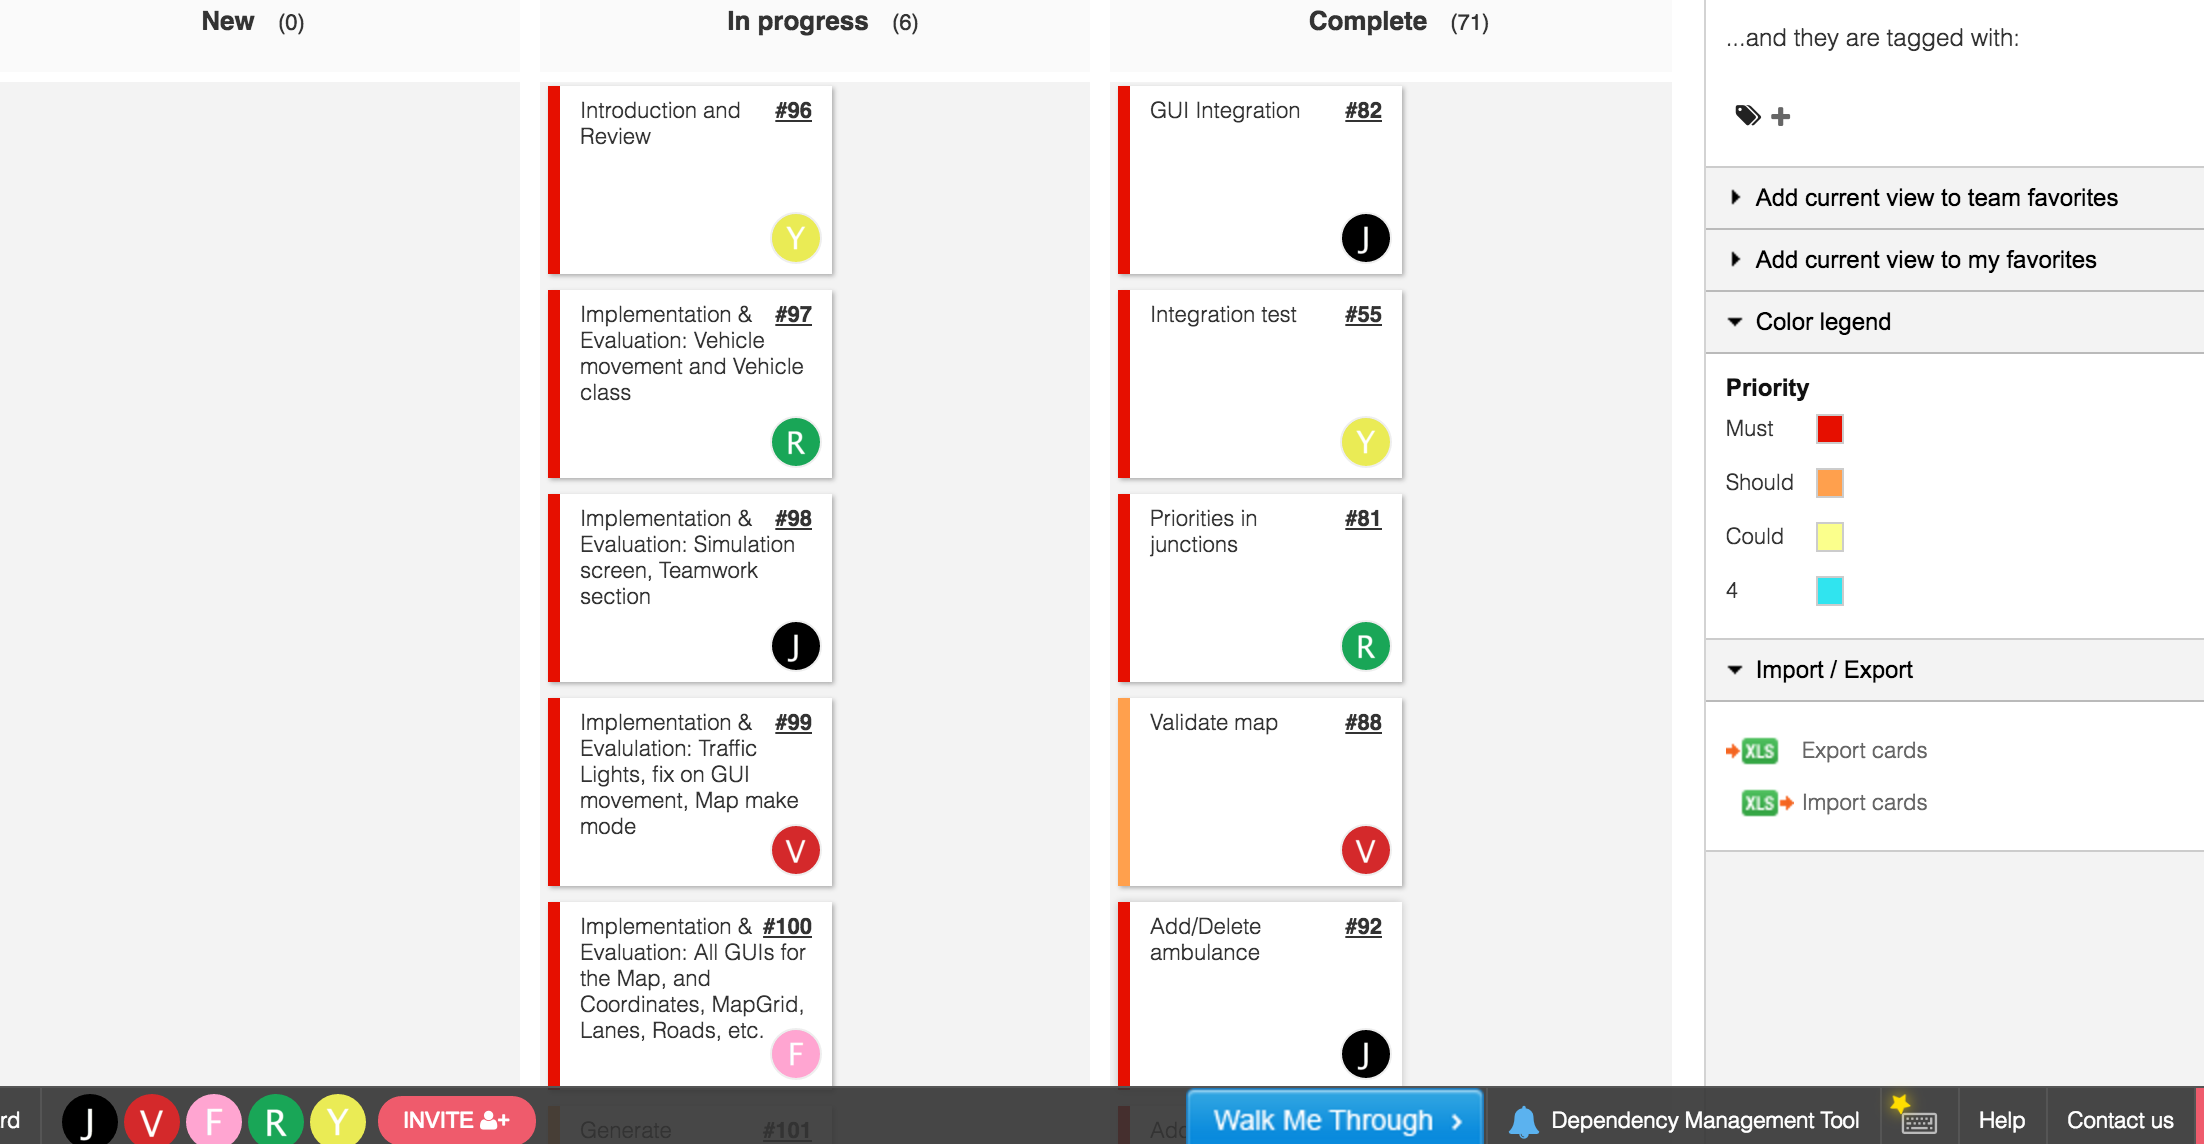
\includegraphics[scale=.15]{mingle1}}
\fbox{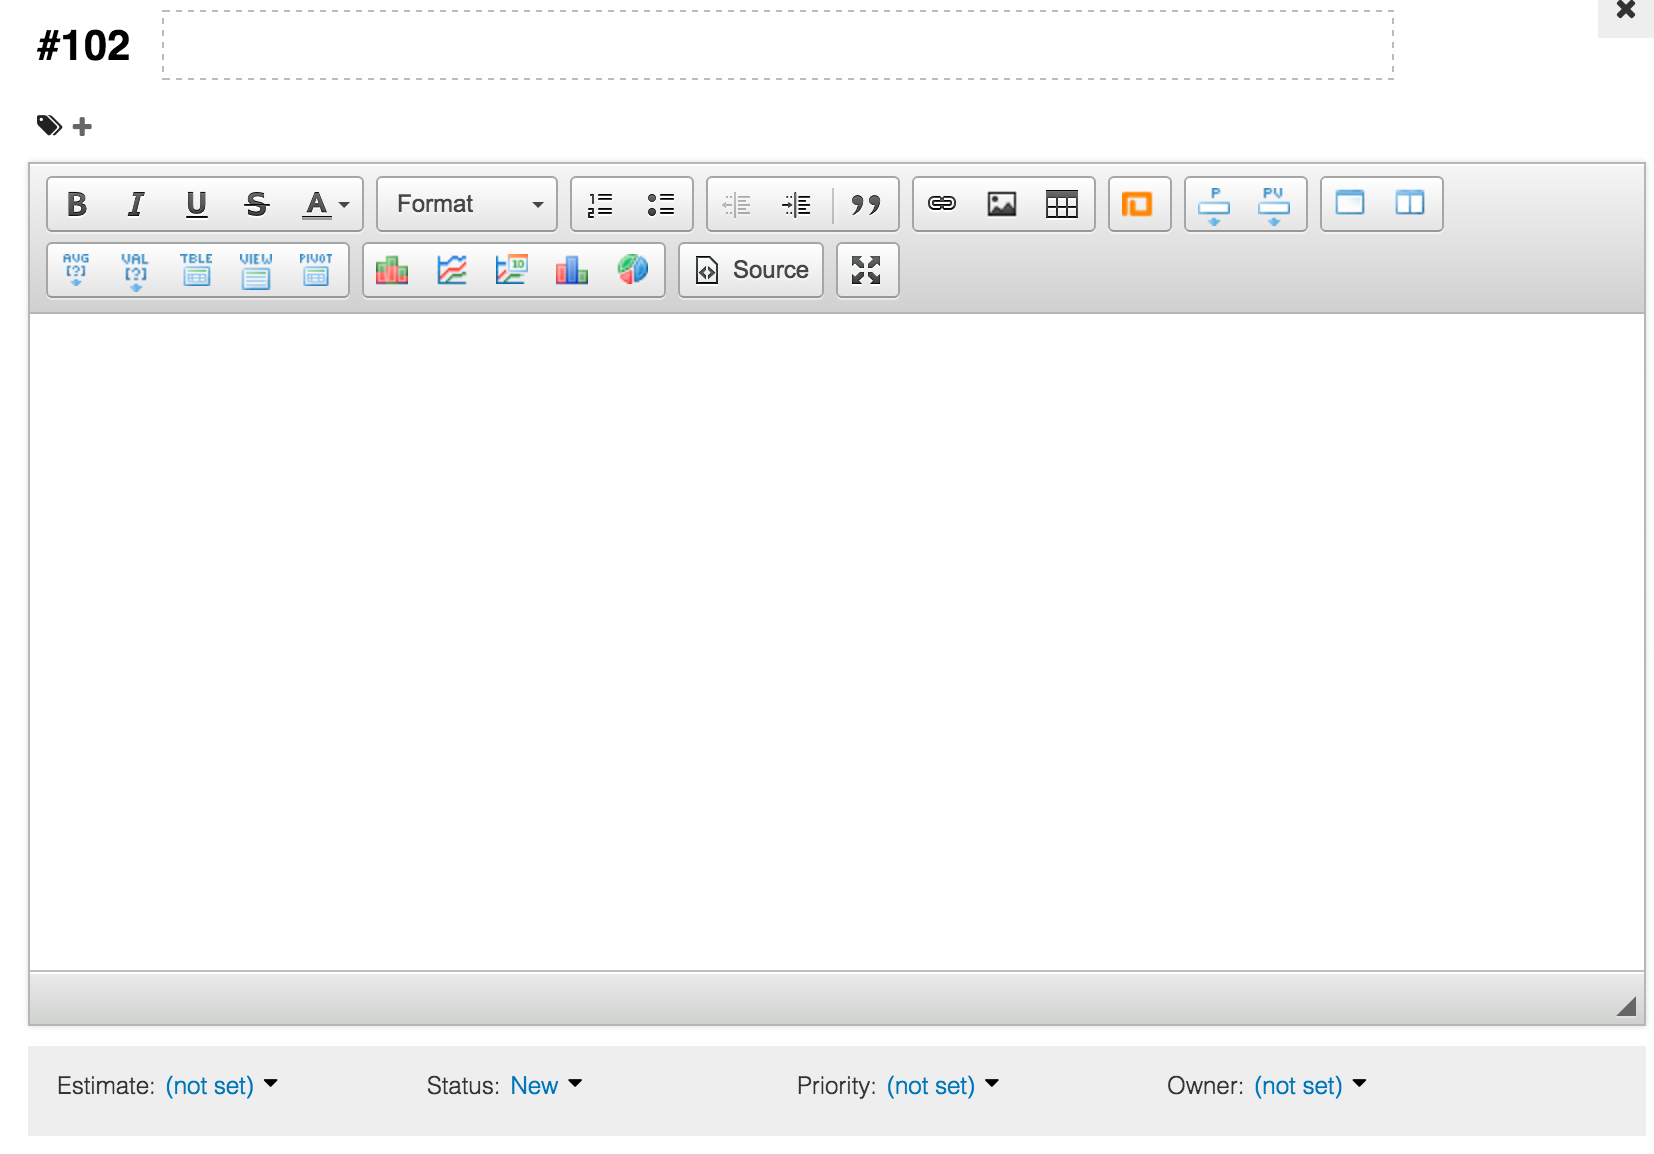
\includegraphics[scale=.15]{mingle2}}
\end{figure}
\end{frame}

\begin{frame}
\frametitle{Simulation Screen}
\begin{itemize}
\item Scene Builder
\item Pure JavaFX 
\begin{itemize}
\item Architecturec: BorderPane
\item Simulaton monitor: Labels
\item Simulation Control: Buttons, slider, dialogs
\begin{figure}[h]

\includegraphics[scale=.35]{JavaFX}
\end{figure}

\end{itemize}
\end{itemize}
\end{frame}

\begin{frame}
\frametitle {General evaluation}
\begin{itemize}
\item Things that went well:
\begin{itemize}
\item project structure
\item teamwork
\item achieved all our goals
\end{itemize}
\item Things that did not go well and what we did:
\begin{itemize}
\item  Ticker, we re-implemented
\item Vehicle movement in maps, we fixed it
\item Loaded maps and traffic lights didn't work, fixed it

\end{itemize}
\item Possiblilities for future:
\begin{itemize}
\item More types of vehicles, roads
\item Curved roads
\item More statistics
\end{itemize}
\end{itemize}

\end{frame}

\begin{frame}
\frametitle {Simulation}
\begin{center}
DEMONSTRATION
\end{center}
\end{frame}

\begin{frame}
\frametitle {Simulation}
\begin{center}
QUESTIONS AND ANSWERS
\end{center}
\end{frame}



\end{document}
